% Generated by build_report.py. Edit the shared content there, then regenerate.
\documentclass[10pt,a4paper]{article}
\usepackage{fontspec}
\setmainfont{texgyretermes}[Extension=.otf,UprightFont=*-regular,BoldFont=*-bold,ItalicFont=*-italic,BoldItalicFont=*-bolditalic]
\usepackage[margin=1.9cm,headheight=14pt]{geometry}
\usepackage{amsmath,amssymb,booktabs,tabularx,longtable,array,ragged2e,enumitem,microtype,xcolor,tikz,fancyhdr,graphicx}
\usetikzlibrary{arrows.meta,positioning}
\usepackage[hidelinks,unicode]{hyperref}
\definecolor{ink}{HTML}{183A45}\definecolor{teal}{HTML}{087F7A}\definecolor{pale}{HTML}{EAF4F2}\definecolor{gray}{HTML}{56656B}
\newcolumntype{P}[1]{>{\RaggedRight\arraybackslash}p{#1}}
\setlength{\parindent}{0pt}\setlength{\parskip}{5pt}\setlength{\emergencystretch}{2em}
\setlength{\tabcolsep}{4pt}\renewcommand{\arraystretch}{1.16}
\setlist{nosep,leftmargin=1.4em,topsep=4pt}
\pagestyle{fancy}\fancyhf{}\fancyhead[L]{\small\color{gray}BẢO VỆ RIÊNG TƯ QUỸ ĐẠO}\fancyhead[R]{\small\color{gray}03/10/2026}\fancyfoot[C]{\small\thepage}\renewcommand{\headrulewidth}{0.3pt}
\newcommand{\key}[1]{\par\smallskip\noindent\colorbox{pale}{\parbox{\dimexpr\linewidth-2\fboxsep}{\textbf{#1}}}\par\smallskip}
\hypersetup{pdftitle={Bảo vệ riêng tư quỹ đạo: dữ liệu, phương pháp và kết quả},pdfauthor={}}
\begin{document}
\begin{center}{\LARGE\bfseries\color{ink}Bảo vệ riêng tư quỹ đạo}\\[5pt]{\large Related works, kiến trúc và kết quả đối chứng}\\[4pt]{\small Bản trình bày rút gọn · 03/10/2026 · Geo-I là phương pháp chính · Hai phiên bản benchmark báo riêng}\end{center}
\section{Related works: scenario và metrics trong một bảng}\label{sec:1}
Khảo sát trong \textbf{21/09/2023–21/09/2026}; $\uparrow$/$\downarrow$ là hướng tốt hơn. Bảng gộp phạm vi scenario và bộ đo của từng paper.

S1: vị trí hiện tại; S2: nơi dừng; S3: đoạn đường đã đi; S4: liên kết danh tính giữa phiên; S5: cạnh đường kế tiếp; S6: đích chưa tới; S7: nội dung/ý định truy vấn; S8: định vị nhờ dữ liệu người đi cùng; S9: điểm đầu bị che; S10: điểm cuối bị che của chuyến đã hoàn tất.

\textbf{Fully:} xử lý trực tiếp nhiệm vụ; \textbf{Partially:} xử lý một phần, trong giả định paper. Đây là đối chiếu của ta, không phải đã vượt mọi ca A/B/C. \textbf{CX:} chưa đủ nguồn; scenario không liệt kê là chưa thấy xử lý trực tiếp (R7/R9: CX; R8/R10: không áp dụng).

\begingroup\small
\begin{longtable}{@{}P{3.044cm}P{1.474cm}P{2.093cm}P{4.138cm}P{5.327cm}@{}}
\toprule
\textbf{Paper} & \textbf{Fully} & \textbf{Partially / CX} & \textbf{Privacy / chẩn đoán} & \textbf{Utility / chi phí}\\\midrule
\endfirsthead
\toprule
\textbf{Paper} & \textbf{Fully} & \textbf{Partially / CX} & \textbf{Privacy / chẩn đoán} & \textbf{Utility / chi phí}\\\midrule
\endhead
\bottomrule\endfoot
TransProtect 2024 [\hyperlink{ref-R1}{R1}] & S1, S3 & S2 & EIE $\uparrow$: sai số suy luận & $\Delta$c $\downarrow$: chênh chi phí hành trình; byte/độ trễ dịch vụ: CX\\
\addlinespace[3pt]
Semantic correlation 2026 [\hyperlink{ref-R2}{R2}] & S1, S3 & S2 & ASR $\uparrow$: đạt ẩn danh; DER $\uparrow$: dummy/ngữ nghĩa & DER chưa đo top-5 POI; thời gian sinh $\downarrow$\\
\addlinespace[3pt]
Fake queries 2026 [\hyperlink{ref-R3}{R3}] & S1, S3 & S2 & Số đường khó phân biệt $\uparrow$; ASR $\uparrow$ & POI: CX; thời gian sinh, RSS $\downarrow$\\
\addlinespace[3pt]
Road-aware PTPPM 2025 [\hyperlink{ref-R4}{R4}] & S1, S3 & S2 & Sai số $\uparrow$; tấn công đúng $\downarrow$ & Dịch chuyển đầu ra $\downarrow$; chi phí LBS: CX (preprint)\\
\addlinespace[3pt]
CPCROK 2025 [\hyperlink{ref-R5}{R5}] & — & S4 & Tỷ lệ khớp quỹ đạo $\rho$ $\downarrow$ & VANET; số quỹ đạo giả $\psi$ $\downarrow$ (chi phí gián tiếp)\\
\addlinespace[3pt]
DP-FETC 2025 [\hyperlink{ref-R6}{R6}] & — & S3, S8, S9, S10 & MI $\downarrow$; bảo đảm $\varepsilon$-DP & JSD phân bố $\downarrow$; độ phức tạp (offline)\\
\addlinespace[3pt]
Improved PIR 2025 [\hyperlink{ref-R7}{R7}] & CX & CX: S1, S7 & Phân tích an toàn; metric tấn công: CX & Truy hồi: CX; tính toán (mới đủ tóm tắt)\\
\addlinespace[3pt]
SoK 2024 [\hyperlink{ref-R8}{R8}] & Không áp dụng & Không áp dụng & Tái dựng/liên kết: nhóm phép đo & Phân bố, hình học, tác vụ (khảo sát)\\
\addlinespace[3pt]
PRISM 2025 [\hyperlink{ref-R9}{R9}] & CX & CX: S1, S3 & LPI: công thức CX & TDD, DC: định nghĩa CX; thời gian xử lý/phản hồi\\
\addlinespace[3pt]
Options to Action 2026 [\hyperlink{ref-R10}{R10}] & Không áp dụng & Không áp dụng & Tỷ lệ dùng tính năng & Nhận thức/sử dụng (nghiên cứu hành vi)\\
\addlinespace[3pt]
Forsch et al. 2023 [\hyperlink{ref-R11}{R11}] & S9, S10 & — & S-TT / k-site-unidentifiability & Che điểm nhạy cảm (tổng quan S-TT 2022)\\
\addlinespace[3pt]
EV querying 2024 [\hyperlink{ref-R12}{R12}] & S1, S3 & S2 & AGeoI + dummy & Truy vấn trạm sạc; phép thử điểm đầu/cuối: CX\\
\end{longtable}
\endgroup
Mốc nền: DLS 2014 [\hyperlink{ref-B1}{B1}], RDG 2021 [\hyperlink{ref-B2}{B2}]. AnotherMe [\hyperlink{ref-B3}{B3}] online 11/09/2023, ngoài cửa sổ dù số tạp chí ghi 2024.

\textbf{Vì sao cần bộ metrics chung?} Điểm số gốc chưa so trực tiếp được vì:

\begin{itemize}
\item \textbf{Đầu ra khác nhau:} vị trí thay thế, quỹ đạo giả, tập dummy hay query chèn. Độ lệch của một điểm công bố chưa cho biết attacker suy được gì từ toàn bộ output.
\item \textbf{Nhiệm vụ và attacker khác nhau:} đo một lần gửi khác đo cả chuỗi hay điểm biên; quyền quan sát, dữ liệu và ngưỡng đánh giá cũng khác.
\item \textbf{Utility khác tác vụ:} giữ phân bố/hình học hoặc dummy hợp ngữ nghĩa chưa đồng nghĩa tìm đúng top-5 POI.
\item \textbf{Chi phí khác phạm vi:} thời gian sinh hay số dummy chưa phản ánh đủ dữ liệu gửi và phản hồi của dịch vụ.
\end{itemize}
\key{Ta dùng Hit100 (\%) $\downarrow$ và MAE (m) $\uparrow$ để chấm cùng đáp án từ toàn bộ output attacker được phép thấy; Recall@5 (\%) $\uparrow$ để đo cùng dịch vụ POI; byte/sự kiện $\downarrow$ để tính request + response. So sánh cùng scenario, dữ liệu và quyền quan sát; kiểm tra Recall mỗi ca $\ge$90\%.}


\clearpage
\section{Kiến trúc mô hình BR-Dummy: Geo-I, mạng đường và các cơ chế}\label{sec:2}
Đọc theo số \textbf{1 $\to$ 2 $\to$ 3a/3b $\to$ 4 $\to$ server $\to$ 5}. Khung xanh là mô hình; A/B là hai cơ chế Boundary tùy chọn.

\begin{center}
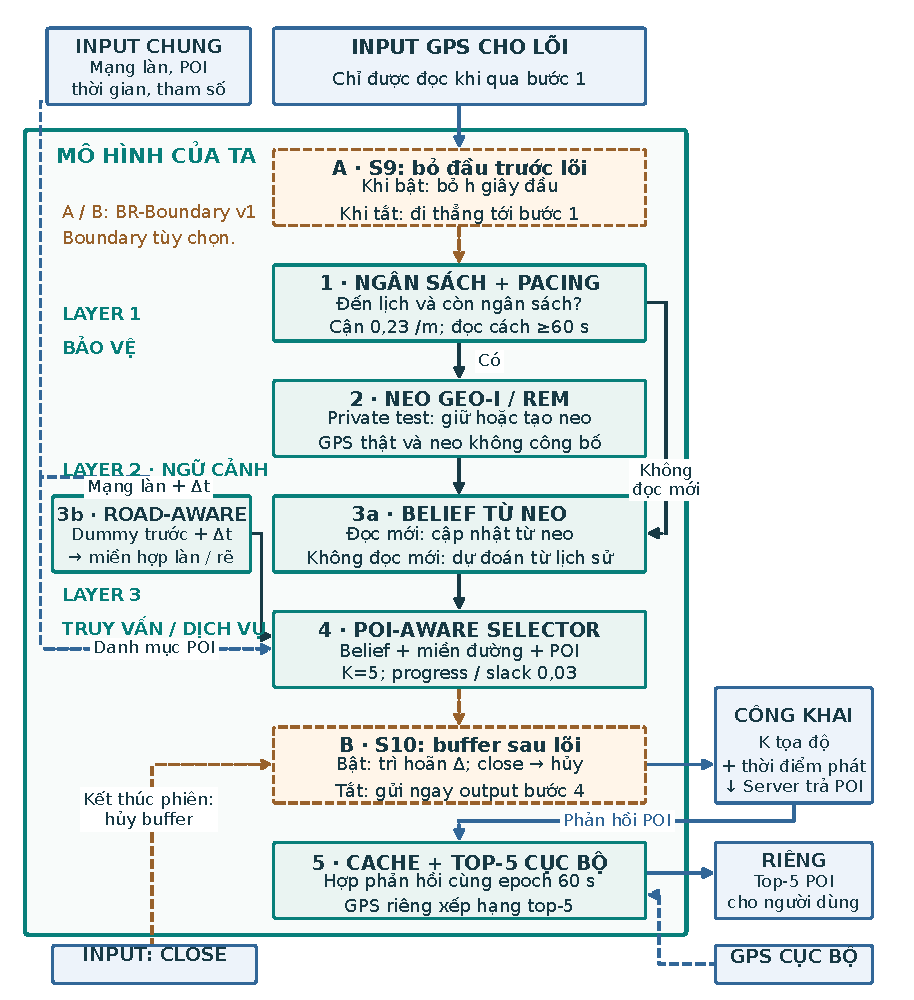
\includegraphics[width=\linewidth,height=0.79\textheight,keepaspectratio]{figures/architecture_report_flow.pdf}
\end{center}
Bước 1 không cho đọc GPS mới thì bỏ qua bước 2. Belief và road-aware cùng đưa đầu vào cho bộ chọn. Cache nhận phản hồi từ server. GPS thật chỉ xếp hạng cục bộ sau khi tạo query.


\clearpage
\subsection{Vai trò các khối và hai cấu hình Geo-I}\label{sub:2.1}
\begingroup\small
\begin{longtable}{@{}P{5.006cm}P{11.913cm}@{}}
\toprule
\textbf{Component} & \textbf{Vai trò trọng tâm}\\\midrule
\endfirsthead
\toprule
\textbf{Component} & \textbf{Vai trò trọng tâm}\\\midrule
\endhead
\bottomrule\endfoot
1. Ngân sách + pacing — S2/S3 & Giới hạn việc đọc GPS trong phiên; giữa các lần đọc chỉ xử lý trạng thái đã bảo vệ.\\
\addlinespace[3pt]
2. Neo Geo-I / REM — S1/S2 & Private test giữ hoặc tạo neo riêng tư; tái dùng giảm mẫu nhiễu mới khi quan sát lặp.\\
\addlinespace[3pt]
3a. Belief từ neo — dịch vụ & Ước lượng vùng vị trí từ lịch sử neo; không coi một neo nhiễu là vị trí chính xác.\\
\addlinespace[3pt]
3b. Road-aware — S3 & Tạo miền dummy tới được theo làn, luật rẽ và thời gian từ dummy bước trước.\\
\addlinespace[3pt]
4. POI-aware selector — dịch vụ & Chọn K query phủ POI bổ sung nhau; progress/slack giúp di chuyển tới vùng phục vụ tốt hơn.\\
\addlinespace[3pt]
5. Cache + top-5 cục bộ — dịch vụ & Hợp phản hồi còn hiệu lực trong epoch; dùng GPS tại thiết bị để xếp hạng top-5.\\
\addlinespace[3pt]
A. Boundary đầu — S9 & Bỏ h giây đầu trước lõi để GPS đoạn này không đi vào trạng thái neo.\\
\addlinespace[3pt]
B. Boundary cuối — S10 & Buffer output sau lõi; khi kết thúc, hủy phần chưa phát thay vì flush.\\
\end{longtable}
\endgroup
Bộ chọn dummy chỉ dùng neo đã bảo vệ và dữ liệu công khai. K dummy không tự tạo k-anonymity. Boundary đã kiểm tra tích hợp, chưa benchmark kết hợp với dịch vụ.

\subsection{Định lượng hai cấu hình Geo-I}\label{sub:2.2}
\textbf{GeoI-Paced:} cấu hình đối chứng nội bộ. \textbf{GeoI-Slack:} bản hiện tại, thêm độ linh hoạt khi chọn dummy. Hai bản cùng ngân sách riêng tư và cùng dịch vụ.

\begingroup\small
\begin{longtable}{@{}P{3.938cm}P{6.350cm}P{6.350cm}@{}}
\toprule
\textbf{Tham số / component} & \textbf{GeoI-Paced} & \textbf{GeoI-Slack}\\\midrule
\endfirsthead
\toprule
\textbf{Tham số / component} & \textbf{GeoI-Paced} & \textbf{GeoI-Slack}\\\midrule
\endhead
\bottomrule\endfoot
Neo / ngân sách & $\varepsilon$\_\allowbreak{}test = $\varepsilon$\_\allowbreak{}release = 0,01 /m; θ = 200 m; cận phiên 0,23 /m & Giống GeoI-Paced\\
\addlinespace[3pt]
Đọc GPS / cache & Đọc cách $\ge$60 giây; cache cùng epoch 60 giây & Giống GeoI-Paced\\
\addlinespace[3pt]
Dịch vụ & K=5 điểm; L=10 POI/loại/điểm; chọn top-5 tại thiết bị & Giống GeoI-Paced\\
\addlinespace[3pt]
Slack & Không nới điểm mục tiêu của bộ chọn & Cho phép giảm tối đa 0,03 điểm mục tiêu để di chuyển hữu ích hơn; không phải giảm Recall 3\%\\
\end{longtable}
\endgroup
\key{Đóng góp: phối hợp lịch sử Geo-I đã bảo vệ, ngân sách, mạng làn và mục tiêu phủ POI. Geo-I + dummy đã có tiền lệ [\hyperlink{ref-R12}{R12}]; lợi ích của cách phối hợp phải được kiểm tra bằng benchmark.}


\clearpage
\section{Benchmark Geo-I: so trực tiếp với đối chứng}\label{sec:3}
\textbf{Benchmark so sánh, phiên bản 2:} K=5, server trả top-5; ba seed, 12 chuyến test. “v2” là phiên bản benchmark, không phải tên attacker. BR tái dùng có cận phiên 0,24 /m; bản trước GeoI-Slack, báo riêng.

\textbf{Cùng tập loại attacker đánh giá mọi phương pháp.} Bộ học như \textbf{Shadow kNN} được huấn luyện riêng từ output mỗi phương pháp. Chọn bộ suy luận theo phương pháp/scenario và chỉ số trên tập chọn, rồi giữ cố định khi test.

\textbf{Attacker thấy gì?} Tọa độ công bố và thời gian trong cửa sổ được phép; biết phương pháp và mạng đường. Không biết điểm thật trong tập dummy, neo nội bộ hay đích ẩn. Đối chứng GPS thật công bố tọa độ thật.

\begingroup\small
\begin{longtable}{@{}P{4.405cm}P{12.514cm}@{}}
\toprule
\textbf{Scenario / đáp án cần suy} & \textbf{Tên các bộ suy luận chính và cách dùng}\\\midrule
\endfirsthead
\toprule
\textbf{Scenario / đáp án cần suy} & \textbf{Tên các bộ suy luận chính và cách dùng}\\\midrule
\endhead
\bottomrule\endfoot
S1 — tọa độ hiện tại & \textbf{Centroid}: tâm tập điểm; \textbf{Prior}: phân bố vị trí; \textbf{Road filter}: lọc đường; \textbf{Shadow kNN}: học từ chuyến phụ trợ.\\
\addlinespace[3pt]
S2 — tọa độ nơi dừng & \textbf{Running mean / Full mean}: gộp nhiều lần nhìn; \textbf{Stationary intersection}: tìm điểm chung khi output có điểm thật + dummy; thêm các bộ đường/chuỗi.\\
\addlinespace[3pt]
S3 — các điểm của đoạn đã đi & \textbf{Continuity}: nối theo chuyển động; \textbf{Road filter}; \textbf{Full path (Viterbi)}: truy ngược toàn cửa sổ; \textbf{Shadow kNN}.\\
\addlinespace[3pt]
S9 — điểm đầu bị che & \textbf{Road filter / Full path} dùng phần tuyến còn thấy; \textbf{Shadow kNN} học quan hệ giữa cửa sổ và điểm đầu.\\
\addlinespace[3pt]
S10 — điểm cuối bị che & \textbf{Road filter / Full path} dùng tuyến trước đoạn bị che; \textbf{Shadow kNN} học quan hệ với điểm cuối; không đọc suffix ẩn.\\
\end{longtable}
\endgroup
\textbf{Cách chọn:} MAE thấp nhất / Hit100 cao nhất trên tập chọn. Tập học, chọn và test dùng xe khác nhau. Tập attacker hữu hạn, chưa bảo đảm tối ưu lý thuyết.

\subsection{So sánh privacy và chất lượng dịch vụ}\label{sub:3.1}
Mỗi ô theo thứ tự \textbf{Hit100 (\%) $\downarrow$ / MAE (m) $\uparrow$ / Recall@5 (\%) $\uparrow$}. Hit100: đoán trong 100 m; MAE: sai số trung bình; Recall: tìm đúng POI. Recall là chỉ số dịch vụ, không phải điểm của attacker.

\begingroup\small
\begin{longtable}{@{}P{2.804cm}P{2.598cm}P{2.598cm}P{2.598cm}P{2.598cm}P{2.598cm}@{}}
\toprule
\textbf{Phương pháp} & \textbf{S1} & \textbf{S2} & \textbf{S3} & \textbf{S9} & \textbf{S10}\\\midrule
\endfirsthead
\toprule
\textbf{Phương pháp} & \textbf{S1} & \textbf{S2} & \textbf{S3} & \textbf{S9} & \textbf{S10}\\\midrule
\endhead
\bottomrule\endfoot
GPS thật & 100,00\% / 13 / 100,00\% & 100,00\% / 39 / 100,00\% & 96,43\% / 23 / 100,00\% & 41,67\% / 120 / 100,00\% & 8,33\% / 630 / 100,00\%\\
\addlinespace[3pt]
DLS* & 58,33\% / 1.318 / 100,00\% & 100,00\% / 39 / 100,00\% & 31,21\% / 1.688 / 100,00\% & 8,33\% / 1.582 / 100,00\% & 0,00\% / 2.029 / 100,00\%\\
\addlinespace[3pt]
TransProtect* & 83,33\% / 84 / 97,78\% & 66,67\% / 88 / 97,19\% & 69,28\% / 99 / 97,93\% & 25,00\% / 184 / 97,27\% & 8,33\% / 680 / 98,52\%\\
\addlinespace[3pt]
Semantic* & 100,00\% / 11 / 100,00\% & 100,00\% / 42 / 100,00\% & 40,58\% / 257 / 100,00\% & 33,33\% / 132 / 100,00\% & 16,67\% / 731 / 100,00\%\\
\addlinespace[3pt]
Geo-I + dummy & 58,33\% / 94 / 99,17\% & 36,11\% / 105 / 98,52\% & 52,65\% / 144 / 97,73\% & 8,33\% / 307 / 96,85\% & 0,00\% / 636 / 97,06\%\\
\addlinespace[3pt]
Geo-I + dummy đường & 16,67\% / 237 / 98,06\% & 53,70\% / 121 / 97,44\% & 3,57\% / 1.909 / 81,96\% & 41,67\% / 217 / 96,99\% & 0,00\% / 2.682 / 79,75\%\\
\addlinespace[3pt]
\textbf{BR tái dùng (Geo-I, v2)} & 33,33\% / 299 / 95,83\% & 22,22\% / 247 / 97,01\% & 7,44\% / 776 / 87,67\% & 0,00\% / 316 / 96,60\% & 0,00\% / 2.315 / 88,33\%\\
\end{longtable}
\endgroup
\key{Ví dụ 33,33\% / 299 / 95,83\%: attacker đoán trong 100 m ở 33,33\% trường hợp; sai số trung bình 299 m; dịch vụ tìm đúng 95,83\% POI chuẩn. Dấu / tách ba chỉ số, không phải phép chia.}

\textbf{Điểm mạnh:} Hit100 S2/S3 thấp hơn ba adapter. \textbf{Đánh đổi:} Recall S3/S10 dưới 90\%; Geo-I + dummy đường có Hit100 S3 tốt hơn nhưng Recall chỉ 81,96\%. DLS có MAE lớn hơn ở S1/S3/S9. Không có phương pháp thắng mọi chỉ số.

* Ba đối chứng là bản thích nghi, không phải tái lập paper. RDG/Fake-query chưa có so trực tiếp cùng protocol; AnotherMe chỉ hoàn thành 11/12 ca S3 nên báo riêng. S9/S10 suy tọa độ đầu/cuối, chưa suy nhãn nhà/nơi làm việc.


\clearpage
\subsection{Bản Geo-I hiện tại: 14 ca và kiểm tra từng component}\label{sub:3.2}
\textbf{Bản hiện tại:} 12 nhóm phát triển, 165 bản ghi từ 94 chuyến; K=5, L=10, cận phiên 0,23 /m. POI khả dụng mô phỏng ở mức 80\%. Hai cột Hit100 so attacker khi thấy GPS thật và khi thấy dữ liệu Geo-I; MAE/Recall là của GeoI-Slack.

\textbf{Ngân hàng attacker ở phép thử này:} \textbf{kNN}, \textbf{ExtraTrees} (cây hồi quy), \textbf{ước lượng hình học} và \textbf{chiếu lên đường}. Đây là bộ đánh giá bổ sung, khác ngân hàng của bảng 3.1. Học trên 64 nhóm phụ trợ, chọn trên 16 nhóm khác, giữ cố định khi chấm 12 nhóm này. S2 gộp chuỗi tại nơi dừng; S3 dùng cả cửa sổ; S9/S10 suy điểm biên, kết hợp chuyến lặp ở S9.C/S10.B. Input chỉ là dữ liệu công bố và thời gian, không thêm GPS/đích thật khi chấm Geo-I.

\begingroup\small
\begin{longtable}{@{}P{1.618cm}P{3.741cm}P{3.741cm}P{3.640cm}P{3.336cm}@{}}
\toprule
\textbf{Ca} & \textbf{GPS thật: Hit100 (\%)} & \textbf{Geo-I: Hit100 (\%) $\downarrow$} & \textbf{Sai số TB (m) $\uparrow$} & \textbf{POI đúng (\%) $\uparrow$}\\\midrule
\endfirsthead
\toprule
\textbf{Ca} & \textbf{GPS thật: Hit100 (\%)} & \textbf{Geo-I: Hit100 (\%) $\downarrow$} & \textbf{Sai số TB (m) $\uparrow$} & \textbf{POI đúng (\%) $\uparrow$}\\\midrule
\endhead
\bottomrule\endfoot
S1.A & 100,00\% & 8,33\% & 852 & 97,64\%\\
\addlinespace[3pt]
S1.B & 100,00\% & 8,33\% & 832 & 95,90\%\\
\addlinespace[3pt]
S1.C & 100,00\% & 0,00\% & 1.674 & 80,18\%\\
\addlinespace[3pt]
S2.A & 100,00\% & 0,00\% & 910 & 99,86\%\\
\addlinespace[3pt]
S2.B & 100,00\% & 4,17\% & 715 & 99,49\%\\
\addlinespace[3pt]
S2.C & 100,00\% & 0,00\% & 997 & 94,59\%\\
\addlinespace[3pt]
S3.A & 100,00\% & 3,09\% & 906 & 95,63\%\\
\addlinespace[3pt]
S3.B & 100,00\% & 3,37\% & 873 & 95,97\%\\
\addlinespace[3pt]
S3.C & 100,00\% & 2,19\% & 934 & 95,26\%\\
\addlinespace[3pt]
S9.A & 16,67\% & 0,00\% & 607 & 95,69\%\\
\addlinespace[3pt]
S9.B & 75,00\% & 2,50\% & 701 & 95,30\%\\
\addlinespace[3pt]
S9.C & 0,00\% & 0,00\% & 514 & 94,95\%\\
\addlinespace[3pt]
S10.A & 33,33\% & 0,00\% & 1.345 & 97,63\%\\
\addlinespace[3pt]
S10.B & 16,67\% & 0,00\% & 1.200 & 96,42\%\\
\end{longtable}
\endgroup
\begingroup\small
\begin{longtable}{@{}P{4.839cm}P{3.581cm}P{3.194cm}P{4.742cm}@{}}
\toprule
\textbf{Cấu hình} & \textbf{POI đúng: Recall@5 $\uparrow$} & \textbf{Ca đạt $\ge$90\%} & \textbf{Byte gửi + nhận / sự kiện $\downarrow$}\\\midrule
\endfirsthead
\toprule
\textbf{Cấu hình} & \textbf{POI đúng: Recall@5 $\uparrow$} & \textbf{Ca đạt $\ge$90\%} & \textbf{Byte gửi + nhận / sự kiện $\downarrow$}\\\midrule
\endhead
\bottomrule\endfoot
GeoI-Paced & 94,38\% & 13/14 & 993,7\\
\addlinespace[3pt]
\textbf{GeoI-Slack} & 95,44\% & 13/14 & 994,1\\
\addlinespace[3pt]
GeoI-Slack, bỏ cache & 95,19\% & 13/14 & 994,1\\
\addlinespace[3pt]
GPS thật & 100,00\% & 14/14 & 214,5\\
\end{longtable}
\endgroup
\key{Kết quả chính: Recall 95,44\%; 13/14 ca đạt ngưỡng. S1.C còn 80,18\%; traffic khoảng 994 byte/sự kiện, so với 214 byte khi gửi GPS thật.}

\textbf{Component:} cache tăng 0,24 điểm \% Recall, không thêm query; khoảng tin cậy 95\% [0,14; 0,34]. Slack tăng 1,06 điểm \%, nhưng khoảng [-0,13; 2,23] chứa 0: chưa chắc chắn. Lấy mẫu lại 12 nhóm, chưa hiệu chỉnh nhiều so sánh.

\textbf{Giới hạn:} Hit100=0 chưa nghĩa là an toàn tuyệt đối. S9.C có Hit100=0 cả với GPS thật; Geo-I vẫn có Hit500=58,33\%. S9/S10 ở đây chưa bật BR-Boundary. Đây là dữ liệu phát triển; cần xác nhận trên nhóm mới.

Recall gộp đều ca trong scenario rồi đều năm scenario. Byte gồm toàn bộ request + response JSON của 94 chuyến, chưa gồm HTTP/TLS/latency. Privacy dùng lại attacker trên cùng tọa độ công bố; cache không đổi query. S10 chỉ A/B, B giữ mã nguồn cũ S10.C.


\clearpage
\section{Phụ lục: đọc chi tiết 14 sample A/B/C}\label{sec:4}
A/B/C là các điều kiện cùng nhiệm vụ, không phải thứ tự độ khó. Mỗi ca chọn một bản ghi thật từ bộ minh họa 12 nhóm/264 chuyến; số bản ghi không phải số chuyến độc lập. \textbf{S10 chỉ có A/B} trong tài liệu; B ánh xạ mã nguồn cũ S10.C để giữ truy nguyên, không có ca C độc lập trong phạm vi hiện tại.

Chấm màu = mẫu trước bảo vệ; nét đứt = đường thật để chấm; sao đỏ = đáp án; trục thời gian tách các mẫu chồng nhau. Đối thủ chỉ nhận dữ liệu đã bảo vệ và thông tin phụ trợ được phép, không nhận các tọa độ/nhãn thật này. Bản đồ minh họa dùng nền SUMO với cùng mã kiểm tra tệp OSM; thiếu mạng gốc để xác minh trùng toàn bộ hình học. © OpenStreetMap contributors.

\subsection{S1 — suy ra vị trí tại một lần gửi}\label{sub:4.1}
Đối thủ cần suy ra tọa độ tại một lần gửi. A/B thay ràng buộc mạng đường; C thêm ngữ cảnh POI hiếm.

\noindent\begin{minipage}[t]{0.48\linewidth}\vspace{0pt}\includegraphics[width=\linewidth]{figures/case_S1_A.pdf}\end{minipage}\hfill\begin{minipage}[t]{0.49\linewidth}\vspace{0pt}\RaggedRight \textbf{S1.A / 12 bản ghi.} Một bản tin tại cạnh có $\ge$2 hướng đi tiếp hợp lệ: kiểm tra khi mạng đường còn nhiều khả năng.\par\smallskip \textbf{Bản ghi minh họa v2-r301-000.} u301\_\allowbreak{}00: 1 mẫu, chỉ số GPS FCD[333…333]\par\smallskip\textbf{Đọc sample.} Một lần lấy mẫu ở cạnh có 4 hướng đi tiếp. Sao đỏ trùng vị trí đầu vào; đối thủ phải chọn vị trí từ đầu ra đã bảo vệ, không được thấy sẵn sao này.\end{minipage}\par\vspace{3pt}
\noindent\begin{minipage}[t]{0.48\linewidth}\vspace{0pt}\includegraphics[width=\linewidth]{figures/case_S1_B.pdf}\end{minipage}\hfill\begin{minipage}[t]{0.49\linewidth}\vspace{0pt}\RaggedRight \textbf{S1.B / 12 bản ghi.} Một bản tin tại cạnh chỉ có 1 hướng đi tiếp: bản đồ tự loại bớt khả năng.\par\smallskip \textbf{Bản ghi minh họa v2-r301-001.} u301\_\allowbreak{}00: 1 mẫu, chỉ số GPS FCD[241…241]\par\smallskip\textbf{Đọc sample.} Vẫn chỉ một lần lấy mẫu, nhưng cạnh chỉ có một hướng đi tiếp. Bản đồ có thể loại bớt khả năng so với A; cần đo lợi thế này bằng đối thủ thực tế.\end{minipage}\par\vspace{3pt}
\noindent\begin{minipage}[t]{0.48\linewidth}\vspace{0pt}\includegraphics[width=\linewidth]{figures/case_S1_C.pdf}\end{minipage}\hfill\begin{minipage}[t]{0.49\linewidth}\vspace{0pt}\RaggedRight \textbf{S1.C / 12 bản ghi.} Cách POI $\le$150 m; loại POI chiếm $\le$5\% danh mục công khai. Hiếm theo loại địa điểm, không phải theo tần suất ghé thăm.\par\smallskip \textbf{Bản ghi minh họa v2-r301-029.} u301\_\allowbreak{}13: 1 mẫu, chỉ số GPS FCD[695…695]\par\smallskip\textbf{Đọc sample.} Điểm lấy mẫu cách POI pharmacy 12,03 m; loại này chiếm 3,11\% danh mục. Ngữ cảnh địa điểm hiếm là dấu hiệu bổ sung, không phải chuỗi di chuyển.\end{minipage}\par\vspace{3pt}

\clearpage
\subsection{S2 — suy ra nơi dừng qua nhiều lần gửi}\label{sub:4.2}
Đối thủ cần suy ra tọa độ nơi dừng. A/B thay thời lượng và nhịp quan sát; C kiểm tra rời đi rồi quay lại.

\noindent\begin{minipage}[t]{0.48\linewidth}\vspace{0pt}\includegraphics[width=\linewidth]{figures/case_S2_A.pdf}\end{minipage}\hfill\begin{minipage}[t]{0.49\linewidth}\vspace{0pt}\RaggedRight \textbf{S2.A / 12 bản ghi.} Dừng có chủ đích $\ge$20 giây; lấy truy vấn mỗi 5 giây.\par\smallskip \textbf{Bản ghi minh họa v2-r301-002.} u301\_\allowbreak{}05: 6 mẫu, chỉ số GPS FCD[54…79]\par\smallskip\textbf{Đọc sample.} 6 mẫu cùng một tọa độ, cách nhau 5 giây; đoạn dừng thật dài 29 giây. Sáu vạch thời gian bị chồng thành một chấm trên map.\end{minipage}\par\vspace{3pt}
\noindent\begin{minipage}[t]{0.48\linewidth}\vspace{0pt}\includegraphics[width=\linewidth]{figures/case_S2_B.pdf}\end{minipage}\hfill\begin{minipage}[t]{0.49\linewidth}\vspace{0pt}\RaggedRight \textbf{S2.B / 12 bản ghi.} Dừng $\ge$120 giây; lấy truy vấn mỗi 20 giây.\par\smallskip \textbf{Bản ghi minh họa v2-r301-003.} u301\_\allowbreak{}06: 9 mẫu, chỉ số GPS FCD[59…219]\par\smallskip\textbf{Đọc sample.} 9 mẫu cùng một tọa độ, cách nhau 20 giây; đoạn dừng dài 179 giây. Đối thủ có cửa sổ dài hơn để kết hợp bằng chứng, không chỉ một bản tin.\end{minipage}\par\vspace{3pt}
\noindent\begin{minipage}[t]{0.48\linewidth}\vspace{0pt}\includegraphics[width=\linewidth]{figures/case_S2_C.pdf}\end{minipage}\hfill\begin{minipage}[t]{0.49\linewidth}\vspace{0pt}\RaggedRight \textbf{S2.C / 12 bản ghi.} Hai lần dừng trên cùng làn, mỗi lần $\ge$20 giây; ở giữa thực sự di chuyển.\par\smallskip \textbf{Bản ghi minh họa v2-r301-004.} u301\_\allowbreak{}07: 18 mẫu, chỉ số GPS FCD[214…1193]\par\smallskip\textbf{Đọc sample.} 18 mẫu chia hai đợt, mỗi đợt 9 mẫu. Hai lần dừng dài 44 giây tại cùng tọa độ; khoảng trống giữa hai cụm thời gian là lúc xe rời đi rồi quay lại.\end{minipage}\par\vspace{3pt}

\clearpage
\subsection{S3 — tái dựng đoạn đường đã đi}\label{sub:4.3}
Đối thủ cần tái dựng các vị trí của đoạn đã đi. A là chuỗi đều; B ít nhánh; C quan sát thưa.

\noindent\begin{minipage}[t]{0.48\linewidth}\vspace{0pt}\includegraphics[width=\linewidth]{figures/case_S3_A.pdf}\end{minipage}\hfill\begin{minipage}[t]{0.49\linewidth}\vspace{0pt}\RaggedRight \textbf{S3.A / 12 bản ghi.} Đoạn di chuyển $\ge$60 giây qua $\ge$3 cạnh; gửi mỗi 20 giây.\par\smallskip \textbf{Bản ghi minh họa v2-r301-005.} u301\_\allowbreak{}00: 12 mẫu, chỉ số GPS FCD[361…581]\par\smallskip\textbf{Đọc sample.} 12 mẫu của u301\_\allowbreak{}00 cách nhau 20 giây. Chuỗi điểm cung cấp nhiều ràng buộc để nối tuyến; nét đứt là đường thật chỉ dùng chấm.\end{minipage}\par\vspace{3pt}
\noindent\begin{minipage}[t]{0.48\linewidth}\vspace{0pt}\includegraphics[width=\linewidth]{figures/case_S3_B.pdf}\end{minipage}\hfill\begin{minipage}[t]{0.49\linewidth}\vspace{0pt}\RaggedRight \textbf{S3.B / 11 bản ghi.} Ít nhất một nửa số cạnh được lấy mẫu chỉ có một hướng đi tiếp: hành lang ít lựa chọn.\par\smallskip \textbf{Bản ghi minh họa v2-r301-007.} u301\_\allowbreak{}00: 9 mẫu, chỉ số GPS FCD[91…251]\par\smallskip\textbf{Đọc sample.} 9 mẫu; 55,6\% cạnh được lấy mẫu chỉ có một hướng đi tiếp. Đường ít nhánh có thể khiến chuỗi dễ suy hơn dù từng vị trí được làm mờ.\end{minipage}\par\vspace{3pt}
\noindent\begin{minipage}[t]{0.48\linewidth}\vspace{0pt}\includegraphics[width=\linewidth]{figures/case_S3_C.pdf}\end{minipage}\hfill\begin{minipage}[t]{0.49\linewidth}\vspace{0pt}\RaggedRight \textbf{S3.C / 12 bản ghi.} Lấy mẫu đoạn di chuyển thưa hơn, mỗi 60 giây.\par\smallskip \textbf{Bản ghi minh họa v2-r301-006.} u301\_\allowbreak{}00: 4 mẫu, chỉ số GPS FCD[361…541]\par\smallskip\textbf{Đọc sample.} 4 mẫu của cùng đoạn trong A, cách nhau 60 giây. Khoảng trống lớn hơn nhưng đối thủ vẫn có thể dùng mạng đường để nối các khả năng.\end{minipage}\par\vspace{3pt}

\clearpage
\subsection{S9 — suy ra điểm xuất phát bị che}\label{sub:4.4}
Đối thủ cần suy điểm đầu bị giấu. A suy ngược một chuyến; B phân biệt hai nguồn nhập tuyến; C kết hợp chuyến lặp.

\noindent\begin{minipage}[t]{0.48\linewidth}\vspace{0pt}\includegraphics[width=\linewidth]{figures/case_S9_A.pdf}\end{minipage}\hfill\begin{minipage}[t]{0.49\linewidth}\vspace{0pt}\RaggedRight \textbf{S9.A / 12 bản ghi.} Cạnh xuất phát chỉ một lối ra. Che 60 giây đầu, lấy phần còn lại mỗi 20 giây.\par\smallskip \textbf{Bản ghi minh họa v2-r301-025.} u301\_\allowbreak{}00: 27 mẫu, chỉ số GPS FCD[60…580]\par\smallskip\textbf{Đọc sample.} Sao là FCD[0]; cửa sổ bắt đầu ở FCD[60] sau khi che 60 giây. Chỉ một lối ra có thể giúp suy ngược nguồn xuất phát từ phần còn công bố.\end{minipage}\par\vspace{3pt}
\noindent\begin{minipage}[t]{0.48\linewidth}\vspace{0pt}\includegraphics[width=\linewidth]{figures/case_S9_B.pdf}\end{minipage}\hfill\begin{minipage}[t]{0.49\linewidth}\vspace{0pt}\RaggedRight \textbf{S9.B / 11 bản ghi.} Hai chuyến khác điểm đầu nhưng nhập một đoạn chung; chỉ cấp từ chỗ nhập tuyến.\par\smallskip \textbf{Bản ghi minh họa v2-r301-026.} u301\_\allowbreak{}00: 28 mẫu, chỉ số GPS FCD[34…574]; u301\_\allowbreak{}04: 28 mẫu, chỉ số GPS FCD[19…559]\par\smallskip\textbf{Đọc sample.} Hai điểm đầu cách 281,76 m rồi nhập tuyến. Chỉ cấp dữ liệu sau nhập; hai sao là hai đáp án bị giấu mà đối thủ phải phân biệt.\end{minipage}\par\vspace{3pt}
\noindent\begin{minipage}[t]{0.48\linewidth}\vspace{0pt}\includegraphics[width=\linewidth]{figures/case_S9_C.pdf}\end{minipage}\hfill\begin{minipage}[t]{0.49\linewidth}\vspace{0pt}\RaggedRight \textbf{S9.C / 12 bản ghi.} Nhiều chuyến có cùng điểm xuất phát dự kiến; che 60 giây đầu từng chuyến.\par\smallskip \textbf{Bản ghi minh họa v2-r301-027.} u301\_\allowbreak{}00: 27 mẫu, chỉ số GPS FCD[60…580]; u301\_\allowbreak{}09: 27 mẫu, chỉ số GPS FCD[60…580]\par\smallskip\textbf{Đọc sample.} u301\_\allowbreak{}00/u301\_\allowbreak{}09 lặp cùng điểm đầu dự kiến; mỗi phiên che 60 giây đầu. Nhiều cửa sổ có thể bổ sung bằng chứng về cùng nguồn xuất phát.\end{minipage}\par\vspace{3pt}

\clearpage
\subsection{S10 — suy ra điểm kết thúc bị che}\label{sub:4.5}
Đối thủ cần suy điểm cuối của chuyến đã hoàn tất. A dùng một chuyến; B kết hợp nhiều chuyến cùng đích. Đây khác dự đoán đích tương lai ở S6.

\noindent\begin{minipage}[t]{0.58\linewidth}\vspace{0pt}\includegraphics[width=\linewidth]{figures/case_S10_A.pdf}\end{minipage}\hfill\begin{minipage}[t]{0.39\linewidth}\vspace{0pt}\RaggedRight \textbf{S10.A / 11 bản ghi.} Cạnh kết thúc chỉ một lối vào. Che 60 giây cuối của chuyến đã hoàn tất.\par\smallskip \textbf{Bản ghi minh họa v2-r302-025.} u302\_\allowbreak{}08: 38 mẫu, chỉ số GPS FCD[0…740]\par\smallskip\textbf{Đọc sample.} Sao là FCD cuối [817] của u302\_\allowbreak{}08; che 60 giây cuối. Đường chỉ một lối vào có thể giúp suy đoạn kết thúc từ phần trước còn thấy.\end{minipage}\par\vspace{3pt}
\noindent\begin{minipage}[t]{0.58\linewidth}\vspace{0pt}\includegraphics[width=\linewidth]{figures/case_S10_B.pdf}\end{minipage}\hfill\begin{minipage}[t]{0.39\linewidth}\vspace{0pt}\RaggedRight \textbf{S10.B / 12 bản ghi.} Nhiều chuyến cùng điểm kết thúc dự kiến; che 60 giây cuối từng chuyến.\par\smallskip \textbf{Bản ghi minh họa v2-r301-028.} u301\_\allowbreak{}00: 27 mẫu, chỉ số GPS FCD[0…520]; u301\_\allowbreak{}09: 27 mẫu, chỉ số GPS FCD[0…520]\par\smallskip\textbf{Đọc sample.} u301\_\allowbreak{}00/u301\_\allowbreak{}09 lặp cùng đích dự kiến và cùng che 60 giây cuối. Đối thủ có thể kết hợp nhiều phiên để khoanh đích, chưa đủ gọi đó là nơi làm việc.\end{minipage}\par\vspace{3pt}
S9/S10 chấm tọa độ đầu/cuối; chưa gán nhãn nhà/nơi làm việc. Xem bản đồ phóng to của 29 ca của khung đầy đủ ở sample\_\allowbreak{}maps.html; tọa độ và bản ghi ở data\_\allowbreak{}samples.json, số đếm ở scenario\_\allowbreak{}inventory.csv.


\clearpage
\section{Nguồn và khả năng truy nguyên}\label{sec:5}
Kết quả so trực tiếp: artifacts/benchmarks/paper\_\allowbreak{}benchmark/results.json và docs/reviews/verification\_\allowbreak{}paper\_\allowbreak{}benchmark\_\allowbreak{}v2.md. Bản mới: iteration18\_\allowbreak{}expanded\_\allowbreak{}attacks.json, iteration28\_\allowbreak{}live\_\allowbreak{}service.json và iteration28\_\allowbreak{}verification.json trong artifacts/benchmarks/research\_\allowbreak{}loop/. geoi\_\allowbreak{}evidence.py kiểm tra hash và gộp lại đúng 14 ca; method\_\allowbreak{}evidence.json lưu nguồn, số đo và bảng đã in. preparation\_\allowbreak{}evidence.json truy nguyên guide. Không chạy thêm mô hình; hai phiên bản được báo riêng.

Ngày 03/10/2026 đưa Geo-I về phương pháp chính; giữ nguyên thực nghiệm gốc và báo riêng hai phiên bản. S10.B là nhãn cho mã nguồn S10.C cũ. Cấu hình, benchmark và phụ lục được dùng chung giữa report/guide; cách dựng và tệp tác giả ở README.md.

\par\hypertarget{ref-R1}{}\textbf{[R1]} Yadav et al. (2024). Protecting Vehicle Location Privacy with Contextually-Driven Synthetic Location Generation (TransProtect). SIGSPATIAL. \href{https://arxiv.org/html/2409.09495v1}{Nguồn gốc}. Toàn văn tác giả; §5.1.4, Eq. 13.
\par\hypertarget{ref-R2}{}\textbf{[R2]} Liu, Peng, Zhou (2026). A Dummy-Based Location Privacy Protection Scheme with Semantic Correlation of Moving Paths. JKSUCIS 38:478. \href{https://link.springer.com/article/10.1007/s44443-026-00899-w}{Nguồn gốc}. Toàn văn NXB; §6.3–6.5.
\par\hypertarget{ref-R3}{}\textbf{[R3]} Liu, Hu, Zhou (2026). Location Privacy Protection in Continuous LBSs: Enhancing Anonymity via Fake Queries. JKSUCIS 38:53. \href{https://link.springer.com/article/10.1007/s44443-025-00438-z}{Nguồn gốc}. Toàn văn NXB; §6.3–6.6.
\par\hypertarget{ref-R4}{}\textbf{[R4]} Road Network-Aware Personalized Trajectory Protection with Differential Privacy under Spatiotemporal Correlations (2025), arXiv:2511.21020v1. \href{https://arxiv.org/html/2511.21020v1}{Nguồn gốc}. Bản tiền công bố; §VI, Eq. 26–27.
\par\hypertarget{ref-R5}{}\textbf{[R5]} Wang et al. (2025). CPCROK: A Communication-Efficient and Privacy-Preserving Scheme for Low-Density Vehicular Ad Hoc Networks. Future Internet 17(4):165. \href{https://uhra.herts.ac.uk/id/eprint/25705/1/futureinternet-17-00165.pdf}{Nguồn gốc}. Toàn văn lưu tại trường tác giả; §5.4.
\par\hypertarget{ref-R6}{}\textbf{[R6]} Yue, Li, Liu, Li (2025). DP-FETC: A differentially private trajectory publishing method based on feature extraction and trajectory correlation. ERA 33(11):6631–6651. \href{https://www.aimspress.com/aimspress-data/era/2025/11/PDF/era-33-11-293.pdf}{Nguồn gốc}. Toàn văn NXB; §4.4, §5.2, Eq. 19–21.
\par\hypertarget{ref-R7}{}\textbf{[R7]} Gu et al. (2025). Research on Joint Protection of LBS Location and Query Privacy in Internet of Vehicles Based on an Improved PIR Algorithm. Concurrency and Computation: Practice and Experience. \href{https://onlinelibrary.wiley.com/doi/abs/10.1002/cpe.70447}{Nguồn gốc}. Chỉ xác minh tóm tắt NXB; chưa đủ định nghĩa các metric.
\par\hypertarget{ref-R8}{}\textbf{[R8]} Buchholz et al. (2024). SoK: Can Trajectory Generation Combine Privacy and Utility? PoPETs 2024(3):75–93. \href{https://petsymposium.org/popets/2024/popets-2024-0068.pdf}{Nguồn gốc}. Toàn văn; khảo sát và hướng dẫn đánh giá, không phải một cơ chế đối chứng.
\par\hypertarget{ref-R9}{}\textbf{[R9]} Farahnakiyan, Esmaeilyfard, Javidan (2025). A proactive privacy-preserving framework for mobile trajectory sharing (PRISM). JNCA 242:104271. \href{https://www.sciencedirect.com/science/article/pii/S1084804525001687}{Nguồn gốc}. Tóm tắt/đoạn công khai của NXB; chưa xác minh công thức LPI/TDD/DC.
\par\hypertarget{ref-R10}{}\textbf{[R10]} Ioannou, Aktypi, Athanasopoulos (2026). From Options to Action: Evaluating Adoption of Privacy Features in Fitness-Tracking Platforms. CHI 2026. \href{https://elathan.github.io/papers/chi26.pdf}{Nguồn gốc}. Toàn văn tác giả; bảng 3, §6.4. Đo sử dụng tính năng, không đo sức chống tấn công.
\par\hypertarget{ref-B1}{}\textbf{[B1]} Niu et al. (2014). Achieving k-Anonymity in Privacy-Aware Location-Based Services (DLS). INFOCOM. \href{https://doi.org/10.1109/INFOCOM.2014.6848002}{Nguồn gốc}. Đối chứng nền; định nghĩa entropy theo hồ sơ khảo sát đã có trong repo.
\par\hypertarget{ref-B2}{}\textbf{[B2]} Shaham et al. (2021). Privacy Preservation in Location-Based Services: A Novel Metric and Attack Model (RDG). IEEE TMC 20(10). \href{https://doi.org/10.1109/TMC.2020.2993599}{Nguồn gốc}. Đối chứng nền; entropy/chuyển tiếp/Viterbi theo hồ sơ đã có trong repo.
\par\hypertarget{ref-B3}{}\textbf{[B3]} Li et al. (2024 issue; online 11/09/2023). AnotherMe: A Location Privacy Protection System Based on Online Virtual Trajectory Generation. IEEE TDSC 21(4):2552–2567. \href{https://ieeexplore.ieee.org/document/10246991/}{Nguồn gốc}. Metadata/tóm tắt và mã nguồn tác giả; chưa kiểm chứng đầy đủ mẫu số/đơn vị phép đo.
\par\hypertarget{ref-B4}{}\textbf{[B4]} Brauer et al. (2022). My home is my secret: concealing sensitive locations by context-aware trajectory truncation. IJGIS 36(12):2496–2524. \href{https://doi.org/10.1080/13658816.2022.2081694}{Nguồn gốc}. Toàn văn NXB và chương tác giả 2023; S-TT, k-site-unidentifiability. Ngoại lệ nền trực tiếp cho S9/S10.
\par\hypertarget{ref-R11}{}\textbf{[R11]} Forsch et al. (2023). Efficient Mining of Volunteered Trajectory Datasets, §3.2. \href{https://link.springer.com/chapter/10.1007/978-3-031-35374-1_3}{Nguồn gốc}. Toàn văn tác giả, online 09/12/2023. Trình bày lại S-TT 2022, không phải một phương pháp mới độc lập.
\par\hypertarget{ref-B5}{}\textbf{[B5]} Dhondt et al. (2022). A Run a Day Won’t Keep the Hacker Away: Inference Attacks on Endpoint Privacy Zones in Fitness Tracking Social Networks. CCS. \href{https://people.cs.kuleuven.be/~stijn.volckaert/papers/2022_CCS_Fitness_Tracking.pdf}{Nguồn gốc}. Bản tác giả: tấn công EPZ và sáu countermeasures; không gắn nhãn một model bảo vệ đã thắng benchmark.
\par\hypertarget{ref-B6}{}\textbf{[B6]} Dehaene et al. (2023). Masking Location Streams in the Presence of Colluding Service Providers. EuroS\&P Workshops. \href{https://lirias.kuleuven.be/bitstream/20.500.12942/720391/2/Data_Stream_Obfuscator_camera_ready.pdf}{Nguồn gốc}. Bản tác giả: Data Stream Obfuscator, privacy zones/timeslots, mapping cache. Tháng 7/2023, ngoài cửa sổ ba năm.
\par\hypertarget{ref-R12}{}\textbf{[R12]} Atmaca et al. (2024). A Privacy-Preserving Querying Mechanism with High Utility for Electric Vehicles. IEEE OJVT. \href{https://wrap.warwick.ac.uk/id/eprint/183198/1/WRAP-privacy-preserving-querying-mechanism-high-utility-electric-vehicles-2024.pdf}{Nguồn gốc}. Bản tác giả: AGeoI + dummy cho truy vấn trạm sạc; không xác minh benchmark điểm đầu/cuối.
\end{document}
